%%%%%%%%%%%%%%%%%%%%%%%%%%%%%%%%%%%%%%%%%
% 
% This template has been adapted by Thomas Höhener to fit the requirements for
% for a PhD-Thesis at the Graduate School for Cellular and Biomedical Sciences
% (GCB) of the University of Bern. 
%
% Check current guidlines on:
% https://www.gcb.unibe.ch/phd_program/phd_thesis_defense__degree/index_eng.html
%
% The template is based on: 
% Masters/Doctoral Thesis 
% LaTeX Template
% Version 2.5 (27/8/17)
%
% This template was downloaded from:
% http://www.LaTeXTemplates.com
%
% Version 2.x major modifications by:
% Vel (vel@latextemplates.com)
%
% This template is based on a template by:
% Steve Gunn (http://users.ecs.soton.ac.uk/srg/softwaretools/document/templates/)
% Sunil Patel (http://www.sunilpatel.co.uk/thesis-template/)
%
% Template license:
% CC BY-NC-SA 3.0 (http://creativecommons.org/licenses/by-nc-sa/3.0/)
%
%%%%%%%%%%%%%%%%%%%%%%%%%%%%%%%%%%%%%%%%%

%----------------------------------------------------------------------------------------
%	PACKAGES AND OTHER DOCUMENT CONFIGURATIONS
%----------------------------------------------------------------------------------------

\documentclass[
11pt, % The default document font size, options: 10pt, 11pt, 12pt
%oneside, % Two side (alternating margins) for binding by default, uncomment to switch to one side
english, % ngerman for German
singlespacing, % Single line spacing, alternatives: onehalfspacing or doublespacing
%draft, % Uncomment to enable draft mode (no pictures, no links, overfull hboxes indicated)
%nolistspacing, % If the document is onehalfspacing or doublespacing, uncomment this to set spacing in lists to single
%liststotoc, % Uncomment to add the list of figures/tables/etc to the table of contents
%toctotoc, % Uncomment to add the main table of contents to the table of contents
%parskip, % Uncomment to add space between paragraphs
%nohyperref, % Uncomment to not load the hyperref package
headsepline, % Uncomment to get a line under the header
%chapterinoneline, % Uncomment to place the chapter title next to the number on one line
%consistentlayout, % Uncomment to change the layout of the declaration, abstract and acknowledgements pages to match the default layout
]{MastersDoctoralThesis} % The class file specifying the document structure

\usepackage[utf8]{inputenc} % Required for inputting international characters
\usepackage[T1]{fontenc} % Output font encoding for international characters

\usepackage{mathpazo} % Use the Palatino font by default

\usepackage[backend=biber,style=authoryear,natbib=true]{biblatex} % Use the bibtex backend with the authoryear citation style (which resembles APA)

\addbibresource{example.bib} % The filename of the bibliography

\usepackage[autostyle=true]{csquotes} % Required to generate language-dependent quotes in the bibliography

\usepackage{svg}
\usepackage[]{hyperref}
\usepackage[nameinlink]{cleveref} % Easy references to Figures, Tables and sections (\cref{})
\usepackage{pdfpages} % insert pdf documents
\usepackage[pagestyles]{titlesec} % remove the prefix ChapterN from the chapter name and in the headers
\titleformat{\chapter}[display]{\normalfont\bfseries}{}{0pt}{\Huge}
\newpagestyle{mystyle}
{\sethead[\thepage][][\chaptertitle]{}{}{\thepage}}
\pagestyle{mystyle}
\setcounter{tocdepth}{2} % adjust depth of TOC: 0-chapter, 1-sectiom, 2-subsection

%----------------------------------------------------------------------------------------
%	MARGIN SETTINGS
%----------------------------------------------------------------------------------------

\geometry{
	paper=a4paper, % Change to letterpaper for US letter
	outer=2.5cm, % Inner margin
	inner=3.8cm, % Outer margin
	bindingoffset=.5cm, % Binding offset
	top=1.5cm, % Top margin
	bottom=1.5cm, % Bottom margin
	%showframe, % Uncomment to show how the type block is set on the page
}

%----------------------------------------------------------------------------------------
%	THESIS INFORMATION
%----------------------------------------------------------------------------------------

% Those information will be used to generate the title page and the abstract. You can also access this information with the corresponding keyword. 

% Keywords used in the template. 
\thesistitle{Production of medically relevant radiolanthanides} % Your thesis title, print it with \ttitle
\supervisor{Prof. Dr. Robert Eichler} % Your supervisor's name, print it with \supname. Include academic title.
\coadvisor{Dr. Zeynep Talip} %Your co-advisors's name, print it with \coaname. Include academic title.
\firstname{Edoardo} % Your first name, print it with \fname. 
\lastname{Renaldin} % Your last name, print it with \lname .
\author{\fname~ \lname} % Your whole name made from your input, print it with \authorname.
\matriculationnumber{22-136-303} % Your matriculation number, print it with \matrnumber
\degree{PhD in Chemistry and Molecular Sciences} % Your degree name, print it with \degreename. 
%Possible degrees at the GCB: PhD in Biochemistry and Molecular Biology, PhD in Cell Biology, PhD in Biomedical Engineering, PhD in Biomedical Sciences, PhD in Immunology, PhD in Neuroscience, Doctor of Medicine and Philosophy (MD,PhD), Doctor of Veterinary Medicine and Philosophy (DVM,PhD), Doctor of Dentistry and Philosophy (DDS,PhD), PhD in Computational Biology, 
\institute{\href{https://www.unibe.ch/}{University of Bern}} % Your department's name and URL, print it with \instname
\faculty{\href{https://www.philnat.unibe.ch/}{Faculty of Science}} % Your department's name and URL, print it with \facname. Possible faculties: Faculty of Medicine, Faculty of Science, Vetsuisse Faculty, Institute of Virology and Immunology IVI, Mittelhäusern, Institute for Research in Biomedicine IRB, Bellinzona
\university{\href{https://www.unibe.ch/}{University of Bern}} % Your university's name and URL, print it with \univname. Possible Universities: University of Bern or University of Zurich (for Vetsuisse Zürich) 

% The following keywords are not used in this template. But define it if you want to use it in the text. 
\department{\href{https://www.dcbp.unibe.ch/}{Department of Chemistry, Biochemistry and Pharmaceutical Sciences}} % Your department's name and URL, print it with \deptname
\group{\href{https://www.GROUP_NAME.net/}{Group name}} % Your research group's name and URL, print it with \groupname
\subject{Radionuclide development} % Your subject area, print it with \subjectname
\keywords{Radiolanthanide, cross section, proton beam} % Keywords for your thesis, print it with \keywordnames


%----------------------------------------------------------------------------------------
%	PDF META DATA
%----------------------------------------------------------------------------------------

\AtBeginDocument{
\hypersetup{pdftitle=\ttitle} % Set the PDF's title to your title
\hypersetup{pdfauthor=\authorname} % Set the PDF's author to your name
\hypersetup{pdfkeywords=\keywordnames} % Set the PDF's keywords to your keywords
}

%----------------------------------------------------------------------------------------
%	DOCUMENT STARTS
%----------------------------------------------------------------------------------------

\begin{document}

\frontmatter % Use roman page numbering style (i, ii, iii, iv...) for the pre-content pages

\pagestyle{plain} % Default to the plain heading style until the thesis style is called for the body content


%----------------------------------------------------------------------------------------
%	TITLE PAGE
%----------------------------------------------------------------------------------------
\begin{titlepage}
{
\vspace*{-3cm}
\hfill

\includegraphics[scale=0.7]{Extra/Logo_UniBe.png} % University logo
}
 \begin{center}
\hypersetup{hidelinks} 
% \vspace*{.08\textheight}
%  {\Large Graduate School for Cellular and Biomedical Sciences\par} % graduate school name
% {\LARGE \univname\par}\vspace{1.5cm} % University name
% \textsc{\Large Doctoral Thesis}\\[0.5cm] % Thesis type

\vspace{3.0cm}
 {\huge \bfseries \ttitle\par}\vspace{.8cm} % Thesis title
  {\Large PhD Thesis submitted by}\\[0.5cm]
  {\LARGE \bfseries \authorname \par}\vspace{0.4cm} % Author name 
  {\Large for the degree of}\\[0.5cm]
  {\Large \degreename \par}

   \vfill

 \emph{Supervisor}\\[1mm]
 {\Large \supname}\\ % Supervisor name
 {\Large \instname}\\ % by default it is your Institute, change if necessary
 {\Large  \facname ~of the \univname} \\% by default it is your Faculty, change if necessary

\vspace{0.4cm}
 \emph{Co-advisor}\\[1mm]
 {\Large \coaname}\\ % Supervisor name
 {\Large \href{https://www.psi.ch/}{Paul Scherrer Institute}}\\
 {\Large \href{https://www.sci.mendel.uni.com/}{Laboratory of Radiochemistry} of the \href{https://www.uni.com/}{Paul Scherrer Institute}}
 
 \vfill
 \end{center}
\end{titlepage}


%----------------------------------------------------------------------------------------
%	Deans PAGE
%----------------------------------------------------------------------------------------
\cleardoublepage
{
\setlength\parindent{0pt} % Remove indent for deans' page
\vspace*{2cm}

Accepted by the Faculty of Medicine, the Faculty of Science and the Vetsuisse Faculty of the University of Bern at the request of the Graduate School for Cellular and Biomedical Sciences \vspace{2cm}

Bern, \hspace{3cm} Dean of the Faculty of Medicine \vspace{3cm}

Bern, \hspace{3cm}Dean of the Faculty of Science \vspace{3cm}

Bern, \hspace{3cm}Dean of the Vetsuisse Faculty Bern

}


%----------------------------------------------------------------------------------------
%	DEDICATORY PAGE
%----------------------------------------------------------------------------------------

\cleardoublepage
\vspace*{0.2\textheight}

\hfill \textit{To all the people in my life who support me so much.}

%----------------------------------------------------------------------------------------
%	QUOTATION PAGE
%----------------------------------------------------------------------------------------

\cleardoublepage
\vspace*{0.2\textheight}

\noindent\enquote{\itshape Science is magic that works.}\bigbreak

\hfill Kurt Vonnegut

%----------------------------------------------------------------------------------------
%	ABSTRACT PAGE
%----------------------------------------------------------------------------------------

\begin{abstract}
\addchaptertocentry{\abstractname} % Add the abstract to the table of contents
The Thesis Abstract is written here (and usually kept to just this page). The page is kept centered vertically so can expand into the blank space above the title too\ldots
\end{abstract}

%----------------------------------------------------------------------------------------
%	ACKNOWLEDGEMENTS
%----------------------------------------------------------------------------------------

\begin{acknowledgements}
\addchaptertocentry{\acknowledgementname} % Add the acknowledgements to the table of contents
The acknowledgments and the people to thank go here, don't forget to include your project advisor\ldots
\end{acknowledgements}

%----------------------------------------------------------------------------------------
%	LIST OF CONTENTS/FIGURES/TABLES PAGES
%----------------------------------------------------------------------------------------

{
  \hypersetup{linkcolor=black} % Make links black in table of content
  \tableofcontents % Prints the main table of contents
  \listoffigures % Prints the list of figures
  \listoftables % Prints the list of tables
}

%----------------------------------------------------------------------------------------
%	ABBREVIATIONS
%----------------------------------------------------------------------------------------

\begin{abbreviations}{ll} % Include a list of abbreviations (a table of two columns)

\textbf{ERK} & \textbf{E}xtracellular signal-\textbf{R}egulated \textbf{K}inases\\

\end{abbreviations}

%----------------------------------------------------------------------------------------
%	THESIS CONTENT - CHAPTERS
%----------------------------------------------------------------------------------------

\mainmatter % Begin numeric (1,2,3...) page numbering

\pagestyle{thesis} % Return the page headers back to the "thesis" style

% Include the chapters of the thesis as separate files from the Chapters folder
% Uncomment the lines as you write the chapters

%\include{Chapters/Chapter0} % Remove this line to remove the Introduction to the template

% Chapter Template

\chapter{Introduction} % Main chapter title
\label{Chapter1} % for referencing this chapter elsewhere, use \cref{Chapter1}
In the recent past decades, the cancer incidence has steadily increased, affecting more than X millions of people. As shown in Figure \ref{fig:asryears}A, the incidence rate has been ever on the rise. Nonetheless, the curve of the mortality rate is dropping since the early 1990s, suggesting more effective treatments have been developed and improved over the last 20 years. Nowadays, several methods are employed to heal this disease: surgery, radiotherapy, chemotherapy, hormone therapy, targeted therapy, immunotherapy and cell-based approaches, and nuclear medicine. To achieve an effective removal of this disease, a combination of these techniques is typically applied to treat the patient. However, 

Figure XB shows both the incidence and mortality rates per 100 000 cases with respect to the body organ affected. 

Tailored treatments is currently the next step to advance further in curing cancer. The cancer relapse still represent the major cause of death. 

\begin{figure}[h!]
	\centering
	
\includegraphics[width=1.0\linewidth]{../Figures/ASR_years}
	\caption{Cancer age-standardized rate (ASR) of European Countries since the beginning of the second half of the 20th century. Data retrieved from GLOBOCAN 2022 (ref).}
	\label{fig:asryears}
\end{figure}


\begin{figure}[h!]
	\raggedright
	
\includegraphics[width=0.7\linewidth]{../Figures/ASR_cancer}
	\caption{Incidence and mortality cancer age-standardized rate (ASR) worldwide grouped according to the organs affected. Data retrieved from GLOBOCAN 2022 (ref).}
	\label{fig:asrcancer}
\end{figure}


\section{Nuclear Medicine}
Intro nuclear medicine

\subsection{Diagnosis}

\subsection{Therapy}
 % Comprehensive introduction into the field

%\include{Chapters/Chapter2}

% Results, can be added as published or submitted manuscripts. If this option is chosen, a separate page needs to be inserted before each manuscript in the thesis, where the title of the manuscript and a short description of your own contribution is stated (i.e., which experiments, which figures are yours).

%\include{Chapters/Chapter3}

% It is only allowed to include published articles in the thesis, if the student is first, shared first, second or shared second author. If the student is third, fourth, fith…. author, a short summary of the publication needs to be done and included in thesis. Please do not forget to cite correctly.

% Overall discussion and outlook/perspectives

%\include{Chapters/Chapter4} 

%----------------------------------------------------------------------------------------
%	THESIS CONTENT - APPENDICES
%----------------------------------------------------------------------------------------

\appendix % Cue to tell LaTeX that the following "chapters" are Appendices

% Include the appendices of the thesis as separate files from the Appendices folder
% Uncomment the lines as you write the Appendices

\include{Appendices/AppendixA}
%\include{Appendices/AppendixB}
%\include{Appendices/AppendixC}

%----------------------------------------------------------------------------------------
%	BIBLIOGRAPHY
%----------------------------------------------------------------------------------------

\printbibliography[heading=bibintoc]


%----------------------------------------------------------------------------------------
%	CV
%----------------------------------------------------------------------------------------
\begin{cvpage}
\phantomsection
\addchaptertocentry{\cv} % Add the cv to the table of contents

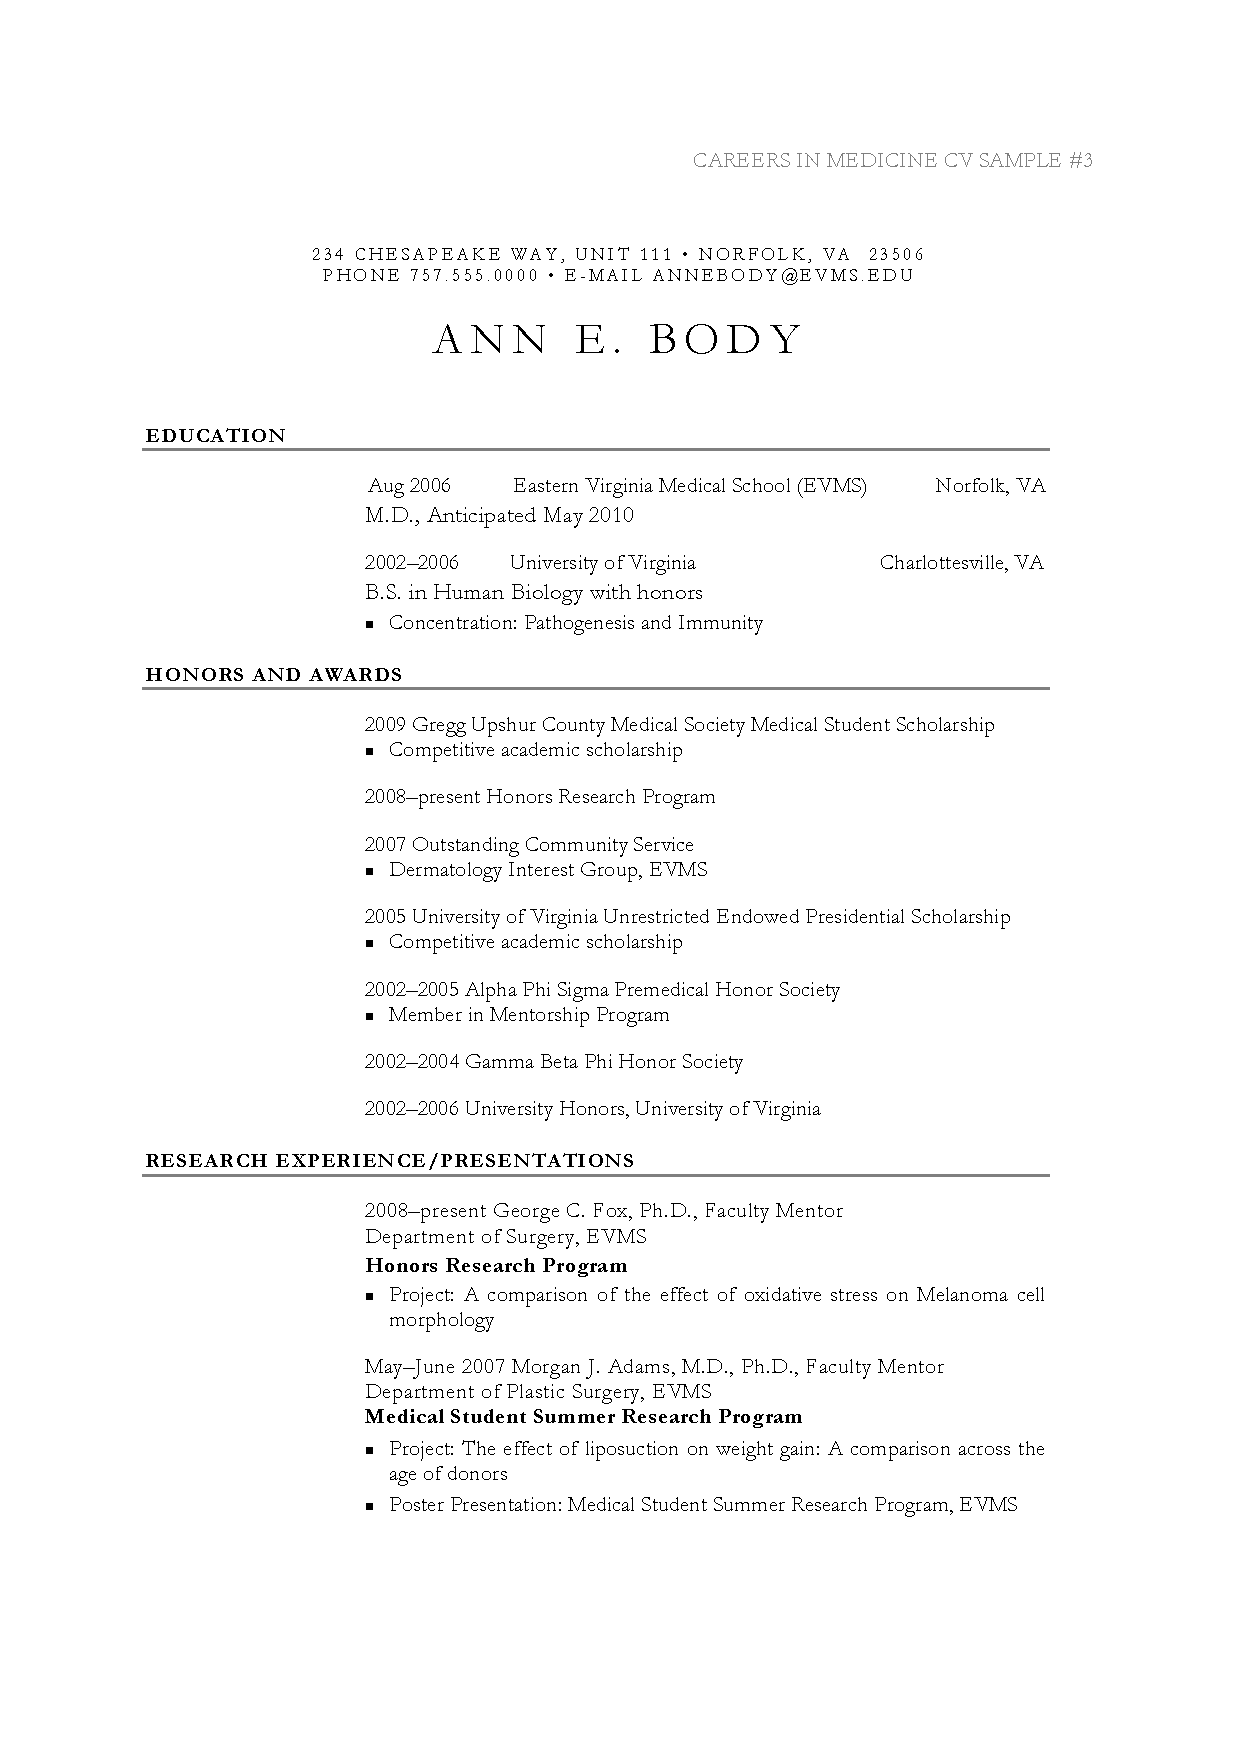
\includepdf[pages=-]{Extra/cv.pdf} % Just replace the cv.pdf file in the "Extra" folder with your own cv. 

\end{cvpage}

%----------------------------------------------------------------------------------------
%	LIST OF PUBLICATIONS
%----------------------------------------------------------------------------------------

\begin{lpubli}
\addchaptertocentry{\publi}
\begin{itemize}


\item \textbf{Smith, J.}, Author, A., Author, B., Author, C., and Author, D., 2022. Your hopefully very awesome paper. \textit{Nature} 4.12 (2022).

\item Author, A., Author, B., \textbf{Smith, J.}, Author, C., and Author, D., 2022. Another very awesome paper you worked on. \textit{Science} 12.53 (2021).

\end{itemize}
\end{lpubli}

\cleardoublepage
%----------------------------------------------------------------------------------------
%	DECLARATION ORIGINALITY
%----------------------------------------------------------------------------------------
% You can either add an electronic signature (just replace the one in figures) or if you prefer, remove the signature, print the page, sign it manually and put a scanned version in the pdf folder. It can den be included with this code: 

%\includepdf[pages=-]{Extra/Declaration_of_Originality.pdf} 


\begin{declaration}
\phantomsection
\addchaptertocentry{\authorshipname} % Add the declaration to the table of contents
\setlength\parindent{0pt} % Remove indent for page

{\noindent\huge\bfseries\authorshipname\par\vspace{10pt}}
\vspace*{5mm}
\textbf{Last name, first name:} \lname, \fname\\[3mm]
\textbf{Matriculation number:} \matrnumber\\[1.2cm]

I hereby declare that this thesis represents my original work and that I have used no other sources except as noted by citations. 
    
All data, tables, figures and text citations which have been reproduced from any other source, including the internet, have been explicitly acknowledged as such. 
    
I am aware that in case of non-compliance, the Senate is entitled to withdraw the doctorate degree awarded to me on the basis of the present thesis, in accordance with the “Statut der Universität Bern (Universitätsstatut; UniSt)”, Art. 69, of 7 June 2011.\\[1.5cm]

Bern, \today\\[4mm]

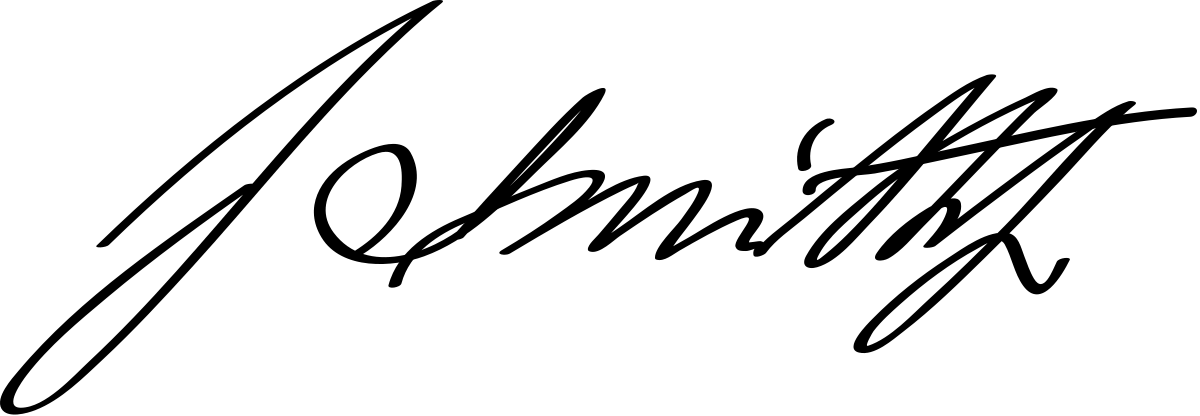
\includegraphics[scale = 0.15]{Extra/signature.png}\\[3mm]
\authorname


\end{declaration}


%----------------------------------------------------------------------------------------

\end{document}  
